\documentclass{article}

\usepackage[latin1]{inputenc}
\usepackage[T1]{fontenc}
\usepackage[francais]{babel}
\usepackage[top = 2cm, bottom = 2cm, left = 2cm, right = 2cm]{geometry}
\usepackage{amssymb,amsfonts,amsthm,amsmath}
\usepackage{graphicx}
\usepackage{multicol}

\newcommand{\R}{\mathbb{R}}

\title{Support Vector Machines Solver}
\author{Jules Pondard - Joseph de Vilmarest}
\date{\today}


\begin{document}

\maketitle

\section*{Introduction}

On cherche � apprendre un classifieur de points dans $\R^n$ en deux cat�gories. On dispose pour cela d'un ensemble d'entra�nement: des points $x_i\in \R^n$ et leur classe $y_i\in\{-1, 1\}$. Un SVM essaie de trouver l'hyperplan s�parateur entre les deux cat�gories optimal, en un certain sens � d�finir.

Formellement, un SVM minimise $\frac{1}{2} \| w \| _2^2 + C1^Tz$ sous les contraintes $z\ge 0$ et $y_i(w^Tx_i)\ge 1-z_i$ pour $1\le i\le m$, en $w\in \R^n$ et $z\in \R^m$.

Durant tout ce rapport on s'int�ressera � un exemple: deux nuages de points de $\R^2$ obtenus comme des gaussiennes de covariance $I_2$ et d'esp�rances respectives $\begin{pmatrix} 0 \\ 0 \end{pmatrix}$ et $\begin{pmatrix} 2 \\ 0 \end{pmatrix}$.


\section{M�thode barri�re}

On applique tout d'abord la m�thode barri�re, en utilisant une m�thode de Newton � chaque pas: on minimise $f(w,x)=t(\frac{w^Tw}{2}+C1^Tz)-\sum\limits_{i=1}^m log(z_i)-\sum\limits_{i=1}^m log(y_i(w^Tx_i)-1+z_i)$ avec un pas $t$ qui tend vers l'infini. On a pris $t=1$ au d�but et on multiplie $t$ par $10$ � chaque �tape.

Pour appliquer la m�thode de Newton, on calcule $\nabla f$ avec
\begin{itemize}
\item[$\bullet$] $\frac{\partial f}{\partial w_i}=tw_i-\sum\limits_{k=1}^m \frac{y_kx_k^i}{y_k(w^Tx_k)-1+z_k}$
\item[$\bullet$] $\frac{\partial f}{\partial z_i}=tC-\frac{1}{z_i}-\frac{1}{y_i(w^Tx_i)-1+z_i}$
\end{itemize}

Pour la hessienne $\nabla ^2 f$, on utilise
\begin{itemize}
\item[$\bullet$] $\frac{\partial ^2 f}{\partial w_i\partial w_j}=t \delta_{i=j}+\sum\limits_{k=1}^m \frac{x_k^ix_k^j}{(y_i(w^Tx_i)-1+z_i)^2}$
\item[$\bullet$] $\frac{\partial ^2 f}{\partial w_i\partial z_j}=\frac{y_jx_j^i}{(y_j(w^Tx_j)-1+z_j)^2}$
\item[$\bullet$] $\frac{\partial ^2 f}{\partial z_i\partial z_j}=\delta_{i=j}(\frac{t}{z_i^2}+\frac{1}{(y_i(w^Tx_i)-1+z_i)^2})$
\end{itemize}

On fait varier C et on affiche, par dessus le nuage de points, la droite s�paratrice trouv�e et la droite "optimale" (m�diatrice des esp�rances des gaussiennes). C'est le graphe de gauche. On afficher de plus le gap � droite.

\newpage
\begin{center}
C=1:
\begin{multicols}{2}
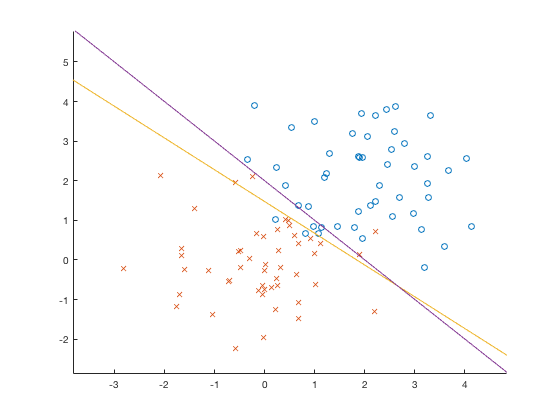
\includegraphics[scale=0.5]{barrier1.png}
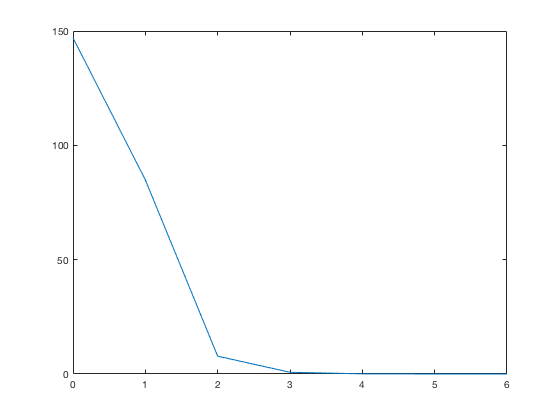
\includegraphics[scale=0.5]{gap1.png}
\end{multicols}

C=100:
\begin{multicols}{2}
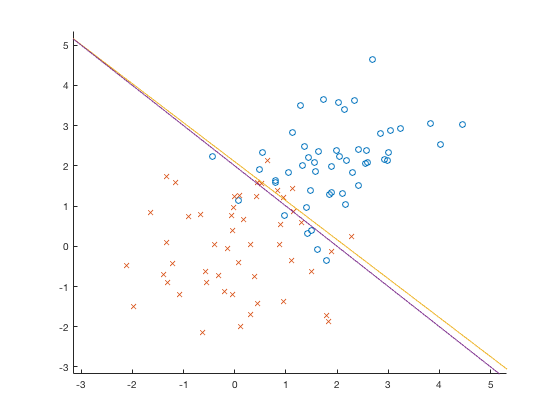
\includegraphics[scale=0.5]{barrier100.png}
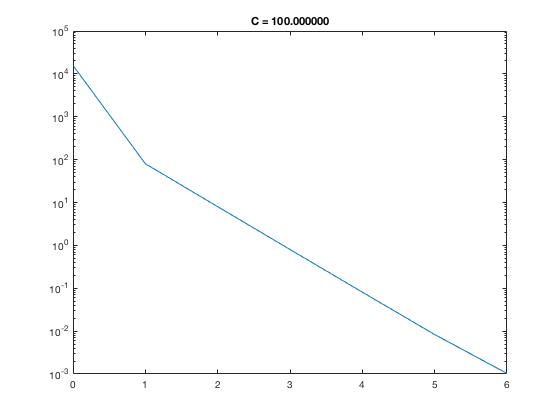
\includegraphics[scale=0.5]{gap100.png}
\end{multicols}
\end{center}

On se rend compte que plus C est grand, plus la solution obtenue est proche de la solution optimale: la p�nalit� $C1^Tz$ est en effet plus importante. On donne ainsi le pourcentage d'erreur sur un ensemble de test en fonction de C. \\

\begin{center}
\begin{tabular}{|c|c|c|c|}
\hline
C & 1 & 10 & 100 \\
\hline
Erreur & & & \\ %a remplir avec matlab
\hline
\end{tabular}
\end{center}


\section{CVX}
%Comparer les performances

On n'a pas r�ussi � utiliser Libsvm qui doit �tre mieux optimis�e pour le probl�me en question.


\end{document}